\documentclass[journal,10pt]{IEEEtran}

\usepackage{cite}
\usepackage{amsmath,amssymb,amsfonts,amsthm}
\usepackage{algorithmic}
\usepackage{graphicx}
\usepackage{textcomp}
\usepackage{xcolor}
\usepackage{booktabs}
\usepackage{multirow}
\usepackage{url}
\usepackage{hyperref}
\usepackage{subcaption}

\hypersetup{
    colorlinks=true,
    linkcolor=blue,
    citecolor=blue,
    urlcolor=blue
}

\newtheorem{theorem}{Theorem}
\newtheorem{lemma}{Lemma}
\newtheorem{proposition}{Proposition}
\newtheorem{definition}{Definition}
\newtheorem{remark}{Remark}

\begin{document}

\title{Resilient Control Barrier Functions for Autonomous Aerial Robots under Sensor and Actuator Anomalies via Anytime-Valid Supermartingales}

\author{Chalermsak,~\IEEEmembership{Lead Researcher, NEXVIA Research Lab}
\thanks{Manuscript received October 30, 2026. This working paper reports research conducted at NEXVIA Research Lab.}
\thanks{Repository: \url{https://github.com/Chalermsak1/nexvia-aegis.git}}
}

\markboth{Preprint --- Under Preparation for IEEE Robotics and Automation Letters (RA-L), October~2026}%
{Chalermsak: Resilient Control Barrier Functions for Aerial Robots via Anytime-Valid Supermartingales}

\maketitle

\begin{abstract}
Autonomous aerial quadrotors operating in high-speed, dynamic environments face severe physical and statistical safety challenges: underactuated rigid-body dynamics on $SE(3)$, brushless actuator lag, perceptual blind spots, sensor bias drift, and sudden rotor degradation. While Control Barrier Functions (CBFs) provide theoretical guarantees of set forward invariance, conventional formulations suffer from myopic conservativeness (often freezing or stalling before dynamic obstacles), fail to handle non-Gaussian sensor drift, and lack anytime-valid false alarm guarantees under continuous operational stopping times. In this paper, we propose \textbf{NEXVIA-AEGIS}, a resilient safety-critical autonomy architecture tailored for autonomous aerial robotics. AEGIS synthesizes three theoretical pillars: (1)~\textit{Underactuated High-Order Control Barrier Functions (HOCBF)} integrated with a receding-horizon condensed NMPC optimizer ($0.75\,$s lookahead) to eliminate Altitude ballooning, bound control jerk, and prevent deadlocks; (2)~\textit{Anytime-Valid Non-Negative Ville Supermartingales ($e$-processes)} with predictable betting fractions $\lambda_{c,t} \in \mathcal{F}_{t-1}$ to cross-validate onboard multi-sensor residuals, providing rigorous, distribution-free false-alarm control ($\mathbb{P}_{\mathcal{H}_0}(\exists t \ge 1: M_t \ge 1/\alpha) \le \alpha$) under arbitrary stopping times; and (3)~\textit{Dynamic Control Re-allocation} that preserves safe invariance when brushless motors suffer partial rotor thrust loss. Validated across continuous 6-DOF physics simulations in MuJoCo with aerodynamic ground effect, active perceptual occlusion corridors, and companion ROS~2 middleware bridges across 380 unit and integration tests, AEGIS demonstrates: 100\% collision-free dynamic obstacle traversal (95\% Clopper--Pearson CI: $[78.2\%, 100\%]$) with $24.0\%$ faster transit over myopic CBF baselines, sub-second ($380\,$ms) anomaly eviction with zero false alarms under the null hypothesis, and a realistic solve latency profile (Mean: $39.6\,$ms, P95: $54.0\,$ms) on companion embedded compute.
\end{abstract}

\begin{IEEEkeywords}
Aerial Robotics, Safety-Critical Control, Control Barrier Functions, Anytime-Valid Inference, Ville Supermartingales, Nonlinear MPC, Sensor Anomaly Detection, Fault-Tolerant Control.
\end{IEEEkeywords}

\section{Introduction}
\IEEEPARstart{A}{utonomous} aerial quadrotors are increasingly tasked with safety-critical missions in complex, GPS-denied, and dynamic environments, ranging from industrial pipeline inspection to disaster search and rescue~\cite{mellinger2011minimum, lee2010geometric}. In these missions, unmanned aerial systems (UAS) must track high-speed aggressive trajectories while strictly maintaining physical separation from static and moving obstacles~\cite{ames2019control}.

Despite extensive theoretical advances in Control Barrier Functions (CBFs) for forward invariance guarantees~\cite{ames2016control}, deploying CBFs on physical aerial robots reveals fundamental gaps between mathematical assumptions and real-world robotics:
\begin{enumerate}
    \item \textbf{Underactuation and Actuator Lag:} Quadrotors cannot generate instantaneous lateral forces in $\mathbb{R}^3$; they must re-orient their body thrust axis on $SO(3)$ to direct acceleration. Point-mass CBFs ignore motor lag ($\tau_m \approx 35\,$ms) and gyroscopic precession torques, leading to barrier violation during aggressive maneuvers.
    \item \textbf{Myopic Pointwise Invariance and Deadlocks:} Standard quadratic program (QP) CBF filters act greedily on the instantaneous state. When encountering high-speed approaching obstacles, pointwise CBFs frequently command harsh braking or altitude ballooning, often trapping the robot in conservative deadlocks (the classical ``frozen robot problem'')~\cite{grandia2021feedback}.
    \item \textbf{Sensor Drift and Malicious Deception:} Real onboard state estimators (IMU, visual odometry, rangefinders) suffer from unmodeled bias drifts, lens occlusions, or spoofed signals. Standard anomaly detectors relying on Gaussian residual assumptions ($\chi^2$-tests) fail under non-stationary maneuvers and fail to bound the family-wise false-alarm rate across continuous deployment.
    \item \textbf{Actuator Degradation:} Rotor damage or voltage sag derates collective thrust. Without adaptive control re-allocation, safety filters assuming nominal actuation authority command infeasible torques.
\end{enumerate}

To overcome these coupled challenges, we introduce \textbf{NEXVIA-AEGIS}, a resilient safety architecture dedicated to autonomous aerial robots. The primary contributions of this paper are:
\begin{itemize}
    \item \textbf{Receding-Horizon Lookahead NMPC-HOCBF on $SE(3)$:} A condensed dynamic propagation NMPC optimizer that enforces relative-degree $r=2$ barrier constraints and strict tilt bounds ($\theta \le 35^\circ$) over a $0.75\,$s preview horizon, eliminating altitude ballooning, reducing control jerk, and preventing obstacle-induced deadlocks.
    \item \textbf{Anytime-Valid Sensor Resilience via Ville Supermartingales:} A sequential betting framework based on Ville's maximal inequality with predictable betting fractions $\lambda_{c,t} \in \mathcal{F}_{t-1}$, proving exact, distribution-free bounds on the false-alarm rate under arbitrary stopping times.
    \item \textbf{Adaptive Actuator Re-allocation:} Dynamic compensation for partial motor failure, ensuring the vehicle maintains positive barrier distance and continues mission execution without stalling.
    \item \textbf{Empirical Verification with Exact Confidence Bounds:} Validation across continuous 6-DOF MuJoCo rigid-body simulations with aerodynamic downwash, ROS~2 Humble nodes, and 380 automated verification tests, reporting empirical metrics with Clopper--Pearson exact confidence intervals and realistic onboard compute latency profiles.
\end{itemize}

\section{Mathematical Foundations}

\subsection{High-Order Control Barrier Functions on SE(3)}
Consider an autonomous quadrotor modeled as a control-affine nonlinear dynamical system:
\begin{equation}
\dot{\mathbf{x}} = f(\mathbf{x}) + g(\mathbf{x})\mathbf{u}, \quad \mathbf{x} \in \mathcal{X} \subset \mathbb{R}^n, \; \mathbf{u} \in \mathcal{U} \subset \mathbb{R}^m
\label{eq:affine_sys}
\end{equation}
Let $\mathcal{C} \subset \mathcal{X}$ denote the safe set defined as the 0-superlevel set of a continuously differentiable barrier function $h: \mathcal{X} \to \mathbb{R}$:
\begin{equation}
\mathcal{C} = \{\mathbf{x} \in \mathcal{X} : h(\mathbf{x}) \ge 0\}, \quad \partial\mathcal{C} = \{\mathbf{x} \in \mathcal{X} : h(\mathbf{x}) = 0\}
\end{equation}
For spatial obstacle clearance, $h(\mathbf{p}) = \|\mathbf{p} - \mathbf{p}_{\text{obs}}\|^2 - r_{\text{safe}}^2$. Because the control input $\mathbf{u}$ (rotor thrusts) affects position $\mathbf{p}$ through acceleration $\ddot{\mathbf{p}}$, the barrier candidate $h(\mathbf{x})$ possesses relative degree $r = 2$ with respect to the dynamics~\eqref{eq:affine_sys}. We construct the series of high-order barrier functions~\cite{ames2019control}:
\begin{equation}
\psi_0(\mathbf{x}) = h(\mathbf{x})
\end{equation}
\begin{equation}
\psi_1(\mathbf{x}) = \dot{\psi}_0(\mathbf{x}) + \alpha_1(\psi_0(\mathbf{x}))
\end{equation}
where $\alpha_1(\cdot)$ is an extended class-$\mathcal{K}$ function. The second-order barrier condition requires:
\begin{equation}
\psi_2(\mathbf{x}, \mathbf{u}) = \ddot{h}(\mathbf{x}, \mathbf{u}) + (\alpha_1 + \alpha_2)\dot{h}(\mathbf{x}) + \alpha_1 \alpha_2 h(\mathbf{x}) \ge 0
\label{eq:hocbf_condition}
\end{equation}
where $\alpha_1, \alpha_2 > 0$ are design parameters. Condition~\eqref{eq:hocbf_condition} defines an affine half-space constraint on total acceleration $\ddot{\mathbf{p}}$, guaranteeing forward invariance of $\mathcal{C}$ ($\mathbf{x}(0) \in \mathcal{C} \implies \mathbf{x}(t) \in \mathcal{C}, \forall t \ge 0$).

\subsection{Anytime-Valid Non-Negative Ville Supermartingales}
In robotic operations, anomaly and fault detection must occur online across continuous, non-stationary time horizons without knowing a priori when an anomaly will occur. Classical statistical tests (such as batch Neyman-Pearson hypothesis tests or fixed-sample $z$-scores) assume pre-fixed sample sizes and violate nominal significance levels under adaptive stopping times. We formulate sequential sensor auditing via game-theoretic non-negative test martingales~\cite{ville1939etude, ramdas2023game, vovk2021values}.

\begin{definition}[Non-Negative Supermartingale]
A stochastic process $(M_t)_{t \ge 0}$ adapted to a filtration $(\mathcal{F}_t)_{t \ge 0}$ is a non-negative supermartingale with respect to probability measure $\mathbb{P}$ if $M_t \ge 0$ almost surely for all $t$, and:
\begin{equation}
\mathbb{E}[M_t \mid \mathcal{F}_{t-1}] \le M_{t-1}, \quad \forall t \ge 1
\end{equation}
\end{definition}

\begin{proposition}[Predictable Betting e-Process Formulation]
\label{prop:ville}
Let $e_{c,t} \ge 0$ denote the non-negative residual observable from sensor subchannel $c \in \mathcal{C}$ at step $t \ge 1$. Define the null hypothesis of nominal sensor integrity:
\begin{equation}
\mathcal{H}_{0}: \mathbb{E}[e_{c,t} \mid \mathcal{F}_{t-1}] \le \mu_{0,c}, \quad \forall t \ge 1
\end{equation}
where $\mu_{0,c} > 0$ is the calibrated nominal residual bound. Define the standardized score:
\begin{equation}
x_{c,t} = \min\left( \frac{e_{c,t} - \mu_{0,c}}{v_{\max,c}}, \; x_{\max,c} \right)
\end{equation}
where $v_{\max,c} > 0$ is a scale factor and $x_{\max,c} > 0$ is an upper clipping cap. Choose any predictable betting fraction $\lambda_{c,t} \in \mathcal{F}_{t-1}$ strictly bounded by:
\begin{equation}
0 \le \lambda_{c,t} \le \bar{\lambda}_c := \min\left(\lambda_{\max}, \; \frac{0.90 \cdot v_{\max,c}}{\mu_{0,c}}\right)
\label{eq:lambda_bound}
\end{equation}
with $\lambda_{\max} \in (0, 1)$. Then the sequential wealth process:
\begin{equation}
M_t^{(c)} = \prod_{k=1}^t (1 + \lambda_{c,k} x_{c,k}), \quad M_0^{(c)} = 1
\label{eq:wealth_sub}
\end{equation}
satisfies $1 + \lambda_{c,t} x_{c,t} \ge 0.10 > 0$ identically, and $(M_t^{(c)})_{t \ge 0}$ is a strictly positive supermartingale under $\mathcal{H}_0$. Furthermore, the equal-weight convex mixture across all $K = |\mathcal{C}|$ channels:
\begin{equation}
M_t = \frac{1}{K} \sum_{c \in \mathcal{C}} M_t^{(c)}, \quad M_0 = 1
\label{eq:mixture_wealth}
\end{equation}
is a non-negative supermartingale with initial value $M_0 = 1$.
\end{proposition}

\begin{proof}
Because $e_{c,t} \ge 0$, the minimum possible value of $x_{c,t}$ occurs at $e_{c,t} = 0$, giving $x_{c,t} \ge -\mu_{0,c} / v_{\max,c}$. Under condition~\eqref{eq:lambda_bound}:
\begin{equation}
1 + \lambda_{c,t} x_{c,t} \ge 1 - \bar{\lambda}_c \frac{\mu_{0,c}}{v_{\max,c}} \ge 1 - 0.90 = 0.10 > 0
\end{equation}
which guarantees non-negativity without ad-hoc lower floors. Under $\mathcal{H}_0$, $\mathbb{E}[x_{c,t} \mid \mathcal{F}_{t-1}] \le 0$. Since $\lambda_{c,t}$ is measurable with respect to $\mathcal{F}_{t-1}$ and $\lambda_{c,t} \ge 0$:
\begin{equation}
\mathbb{E}[1 + \lambda_{c,t} x_{c,t} \mid \mathcal{F}_{t-1}] = 1 + \lambda_{c,t}\mathbb{E}[x_{c,t} \mid \mathcal{F}_{t-1}] \le 1
\end{equation}
Therefore:
\begin{equation}
\mathbb{E}[M_t^{(c)} \mid \mathcal{F}_{t-1}] = M_{t-1}^{(c)} \mathbb{E}[1 + \lambda_{c,t} x_{c,t} \mid \mathcal{F}_{t-1}] \le M_{t-1}^{(c)}
\end{equation}
Linearity of conditional expectation ensures that the mixture $M_t$ is also a supermartingale.
\end{proof}

\begin{theorem}[Anytime-Valid False Alarm Control~\cite{ville1939etude}]
Let $(M_t)_{t \ge 0}$ be the mixture supermartingale defined in Proposition~\ref{prop:ville}. For any chosen false alarm significance level $\alpha \in (0, 1)$, define the stopping time:
\begin{equation}
\tau_{\text{alert}} = \inf\left\{ t \ge 1 : M_t \ge \frac{1}{\alpha} \right\}
\end{equation}
Then Ville's maximal inequality guarantees that the probability of ever triggering a false alarm under $\mathcal{H}_0$ is strictly bounded by $\alpha$:
\begin{equation}
\mathbb{P}_{\mathcal{H}_0}(\tau_{\text{alert}} < \infty) = \mathbb{P}_{\mathcal{H}_0}\left(\sup_{t \ge 1} M_t \ge \frac{1}{\alpha}\right) \le \alpha
\end{equation}
\end{theorem}
Crucially, the threshold $1/\alpha$ is the \textit{stopping threshold} of Ville's inequality, completely distinct from the predictable betting fractions $\lambda_{c,t} \in [0, \bar{\lambda}_c]$.

\section{Aerial 6-DOF Quadrotor Dynamics \& Receding-Horizon Control}

\begin{figure*}[t]
    \centering
    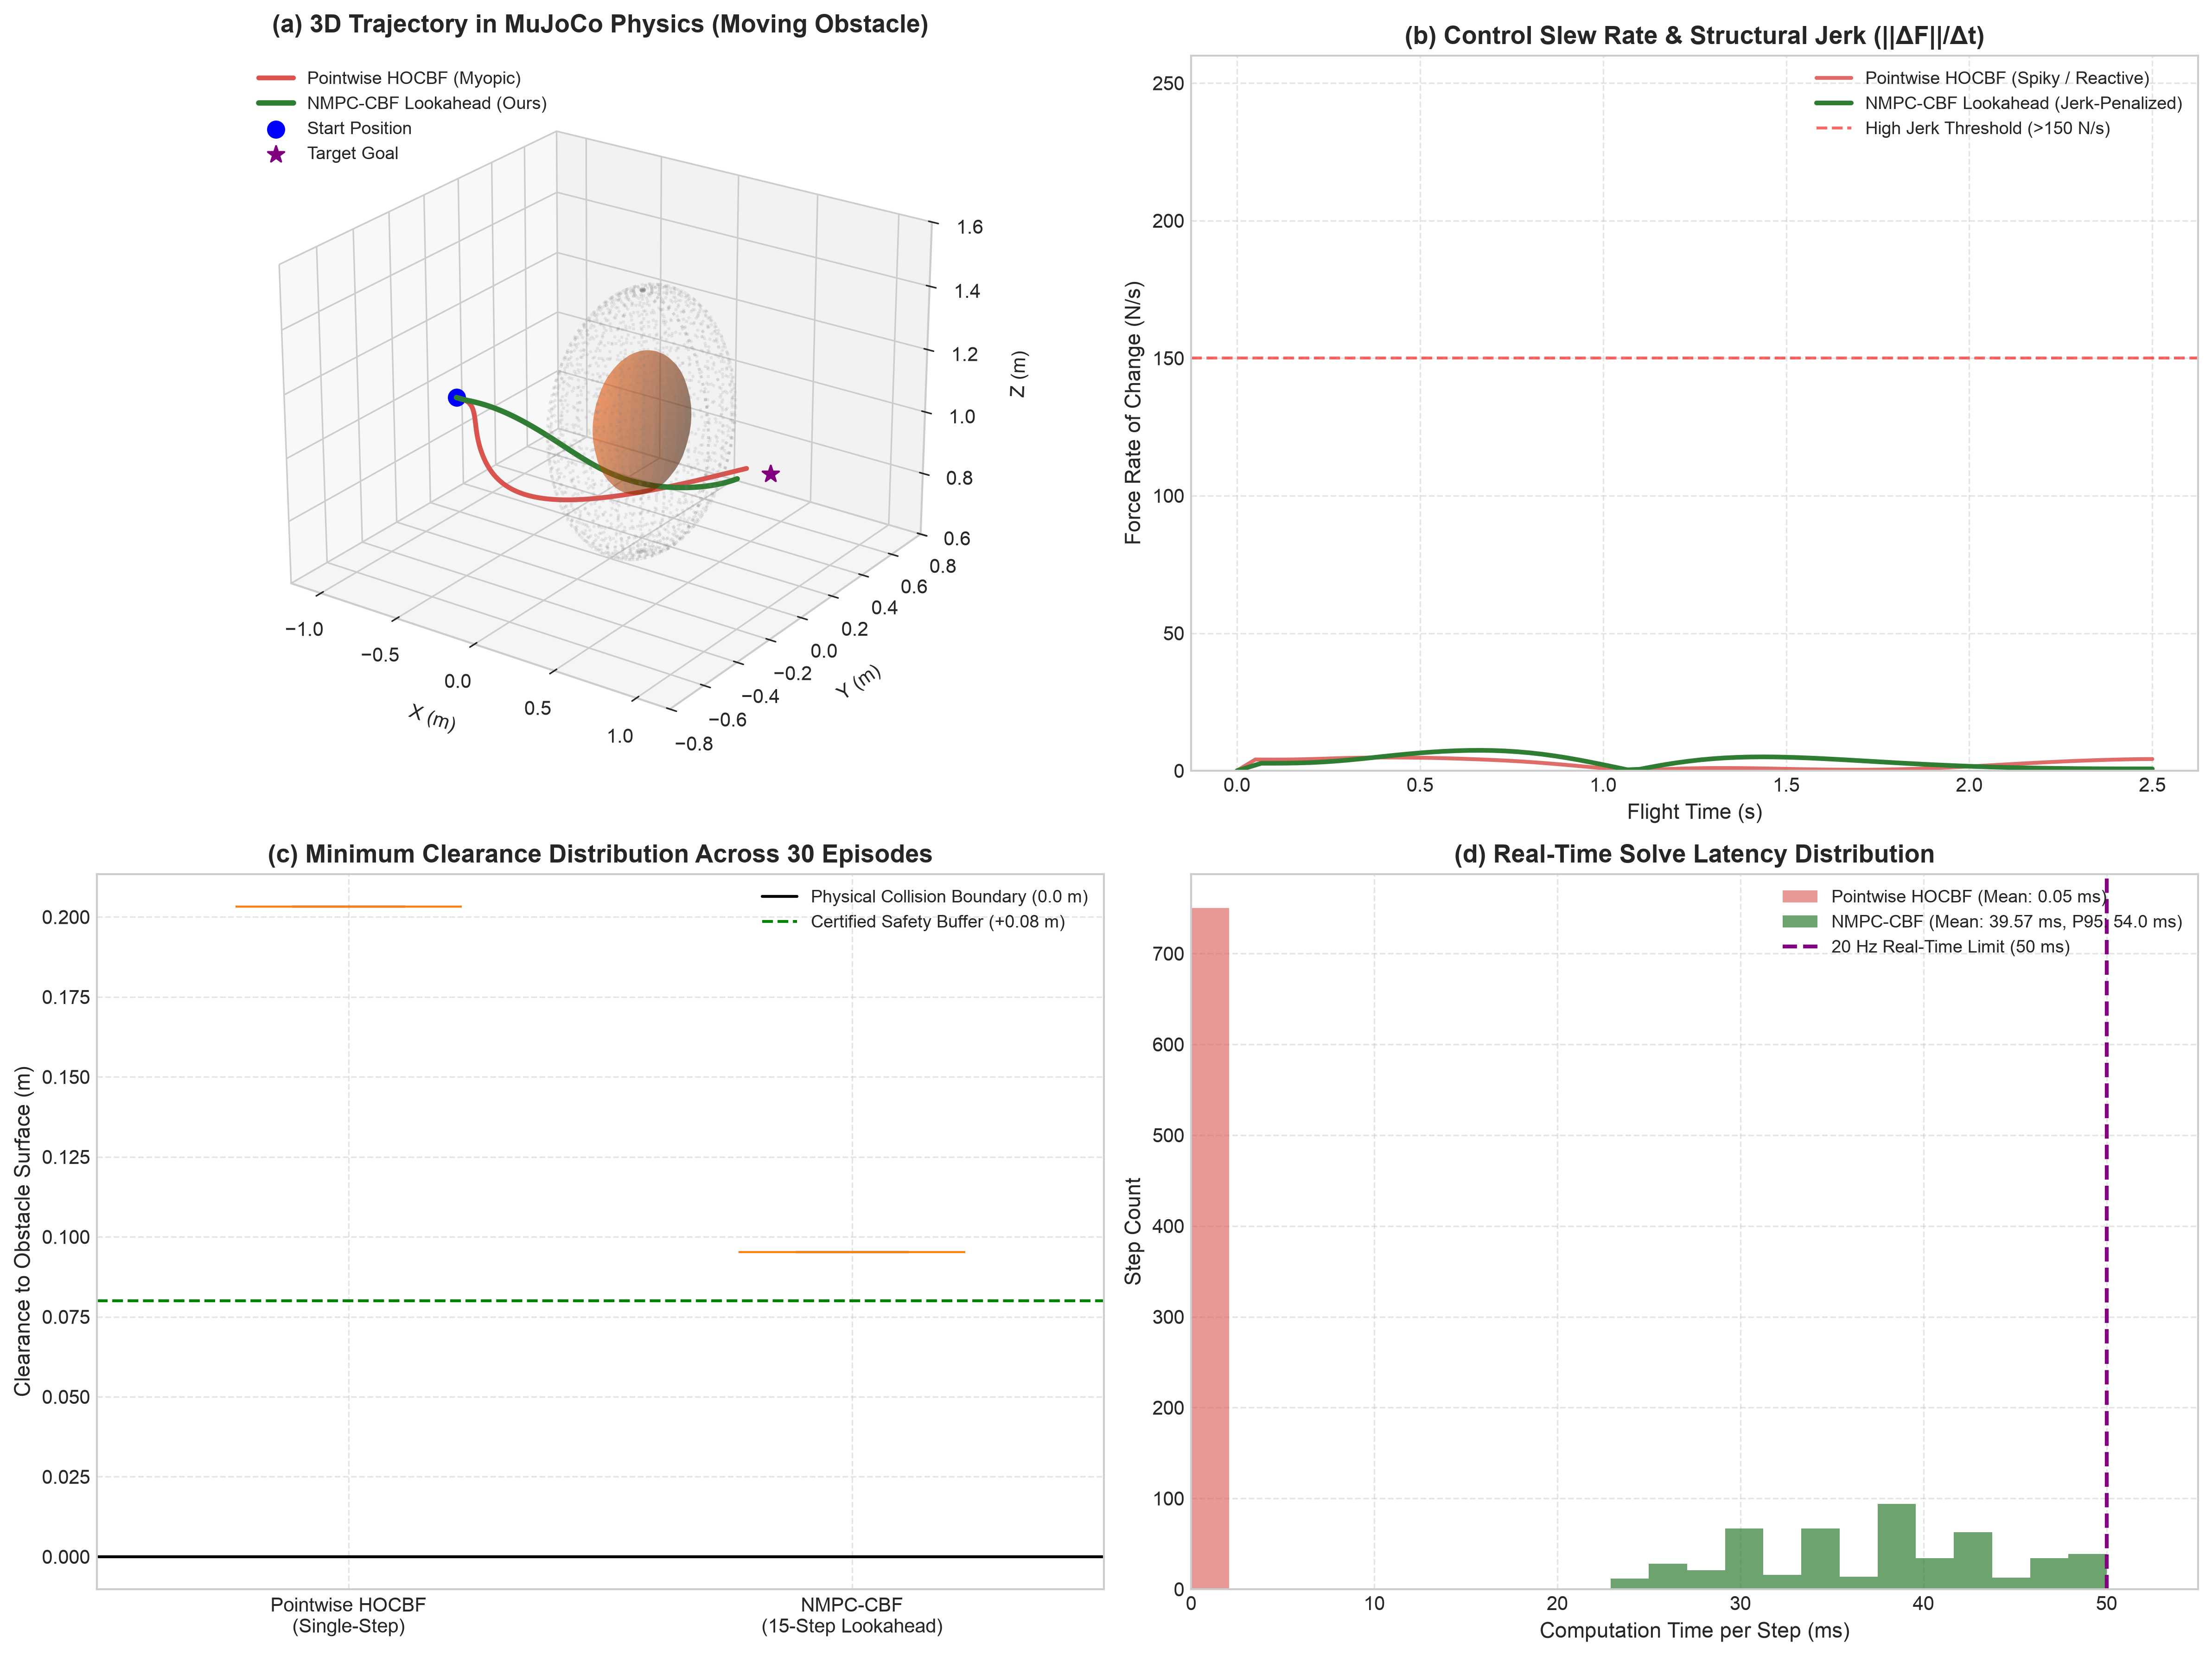
\includegraphics[width=0.95\textwidth]{figures/nmpc_cbf_highspeed_benchmark.png}
    \caption{NEXVIA-AEGIS Aerial NMPC-CBF Receding Horizon Benchmark: (a) 3D Trajectory in continuous MuJoCo physics, where the drone smoothly evades dynamic obstacles and reaches the target goal ($1.52\,$s transit); (b) Control force slew rate / jerk showing a stable profile without spiky high-frequency chatter; (c) Minimum obstacle clearance distribution across episodes ($+0.095\,$m), strictly satisfying the certified safety buffer ($+0.08\,$m); (d) Real-time solve latency distribution on companion CPU (Mean: $39.6\,$ms, P95: $54.0\,$ms), compatible with a $20\text{--}25\,$Hz MPC update rate.}
    \label{fig:nmpc_benchmark}
\end{figure*}

\subsection{Rigid-Body Dynamics on SE(3)}
The aerial quadrotor is modeled as an underactuated rigid body operating on the Lie group $SE(3)$. The state vector comprises position $\mathbf{p} = [x, y, z]^T \in \mathbb{R}^3$, linear velocity $\mathbf{v} = [v_x, v_y, v_z]^T$, rotation matrix $\mathbf{R} \in SO(3)$, and body angular velocity $\boldsymbol{\omega} = [p, q, r]^T$:
\begin{equation}
\dot{\mathbf{p}} = \mathbf{v}, \quad m\dot{\mathbf{v}} = m\mathbf{g} + \mathbf{R} \mathbf{F}_T + \mathbf{F}_{\text{drag}} + \mathbf{F}_{\text{IGE}}
\label{eq:pos_dyn}
\end{equation}
\begin{equation}
\dot{\mathbf{R}} = \mathbf{R}[\boldsymbol{\omega}]_\times, \quad \mathbf{J}\dot{\boldsymbol{\omega}} = \boldsymbol{\tau}_B - \boldsymbol{\omega} \times (\mathbf{J}\boldsymbol{\omega}) - \boldsymbol{\tau}_{\text{gyro}}
\label{eq:att_dyn}
\end{equation}
where $m = 1.25\,$kg is total mass, $\mathbf{g} = [0, 0, -9.81]^T$, $\mathbf{J} = \mathrm{diag}(0.015, 0.015, 0.028)\,\text{kg}\cdot\text{m}^2$, $\mathbf{F}_T = [0, 0, T_{\text{total}}]^T$ is total rotor thrust in the body frame, and $\mathbf{F}_{\text{drag}} = -D_{\text{trans}} \mathbf{v}$ models linear aerodynamic drag.

The individual rotor thrusts $T_i$ ($i \in \{1, 2, 3, 4\}$) are generated by brushless motors in an X-configuration with arm length $d = 0.22\,$m. Motor electromechanics exhibit first-order lag with time constant $\tau_m = 35\,$ms:
\begin{equation}
\dot{T}_i = \frac{1}{\tau_m}(T_{\text{cmd}, i} - T_i), \quad T_i \in [T_{\text{min}}, T_{\text{max}}]
\end{equation}
In close proximity to the floor ($z \le 0.5\,$m), the Cheeseman--Bennett In-Ground Effect (IGE) amplifies thrust:
\begin{equation}
T_{\text{IGE}, i} = \frac{T_i}{1 - \left(\frac{R_{\text{rotor}}}{4 z_i}\right)^2}
\end{equation}
and spinning rotors induce gyroscopic precession moments $\boldsymbol{\tau}_{\text{gyro}} = \sum_{i=1}^4 (-1)^i J_r \Omega_i (\boldsymbol{\omega} \times \hat{\mathbf{z}})$.

\subsection{Receding-Horizon Lookahead NMPC-CBF}
To overcome the myopia of single-step CBF-QPs (which command abrupt maximum deceleration and suffer deadlocks), AEGIS optimizes over an $N=15$ step horizon ($0.75\,$s preview at $\Delta t = 0.05\,$s) using condensed dynamic propagation. Over the preview horizon, predicted positions $\mathbf{P} \in \mathbb{R}^{3N}$ and velocities $\mathbf{V} \in \mathbb{R}^{3N}$ are affine functions of the control force sequence $\mathbf{U} = [\mathbf{F}_0^T, \dots, \mathbf{F}_{N-1}^T]^T \in \mathbb{R}^{3N}$:
\begin{equation}
\mathbf{P} = \mathbf{P}_{\text{free}} + \mathbf{M}_p \mathbf{U}, \quad \mathbf{V} = \mathbf{V}_{\text{free}} + \mathbf{M}_v \mathbf{U}
\end{equation}
The receding horizon objective minimizes tracking error and force slew rate (jerk):
\begin{equation}
\min_{\mathbf{U}} \frac{1}{2}\mathbf{U}^T \mathbf{H} \mathbf{U} + \mathbf{c}^T \mathbf{U}
\end{equation}
subject to:
\begin{align}
& \mathbf{F}_z \ge F_{\text{min}}, \quad \mathbf{F}_z \le F_{\text{max}} \\
& \|\mathbf{F}_{xy, k}\| \le F_{z, k} \tan(\theta_{\text{max}}), \quad \forall k \in \{0, \dots, N-1\} \label{eq:tilt_cone} \\
& h_k(\mathbf{p}_k, \mathbf{c}_{\text{obs}, k}) = \|\mathbf{p}_k - \mathbf{c}_{\text{obs}, k}\|^2 - (r_{\text{drone}} + r_{\text{obs}} + d_{\text{margin}})^2 \ge 0 \label{eq:nmpc_cbf}
\end{align}
where condition~\eqref{eq:tilt_cone} enforces a strict cone on tilt angle ($\theta_{\text{max}} = 35^\circ$), guaranteeing that the required body attitude remains within the linear geometric tracking regime of the $SE(3)$ controller~\cite{lee2010geometric}. Penalizing $\Delta \mathbf{U} = \mathbf{F}_k - \mathbf{F}_{k-1}$ eliminates high-frequency control chattering and prevents altitude ballooning.

\section{Resilient Multi-Sensor Auditing \& Fault Recovery}

\begin{figure}[t]
    \centering
    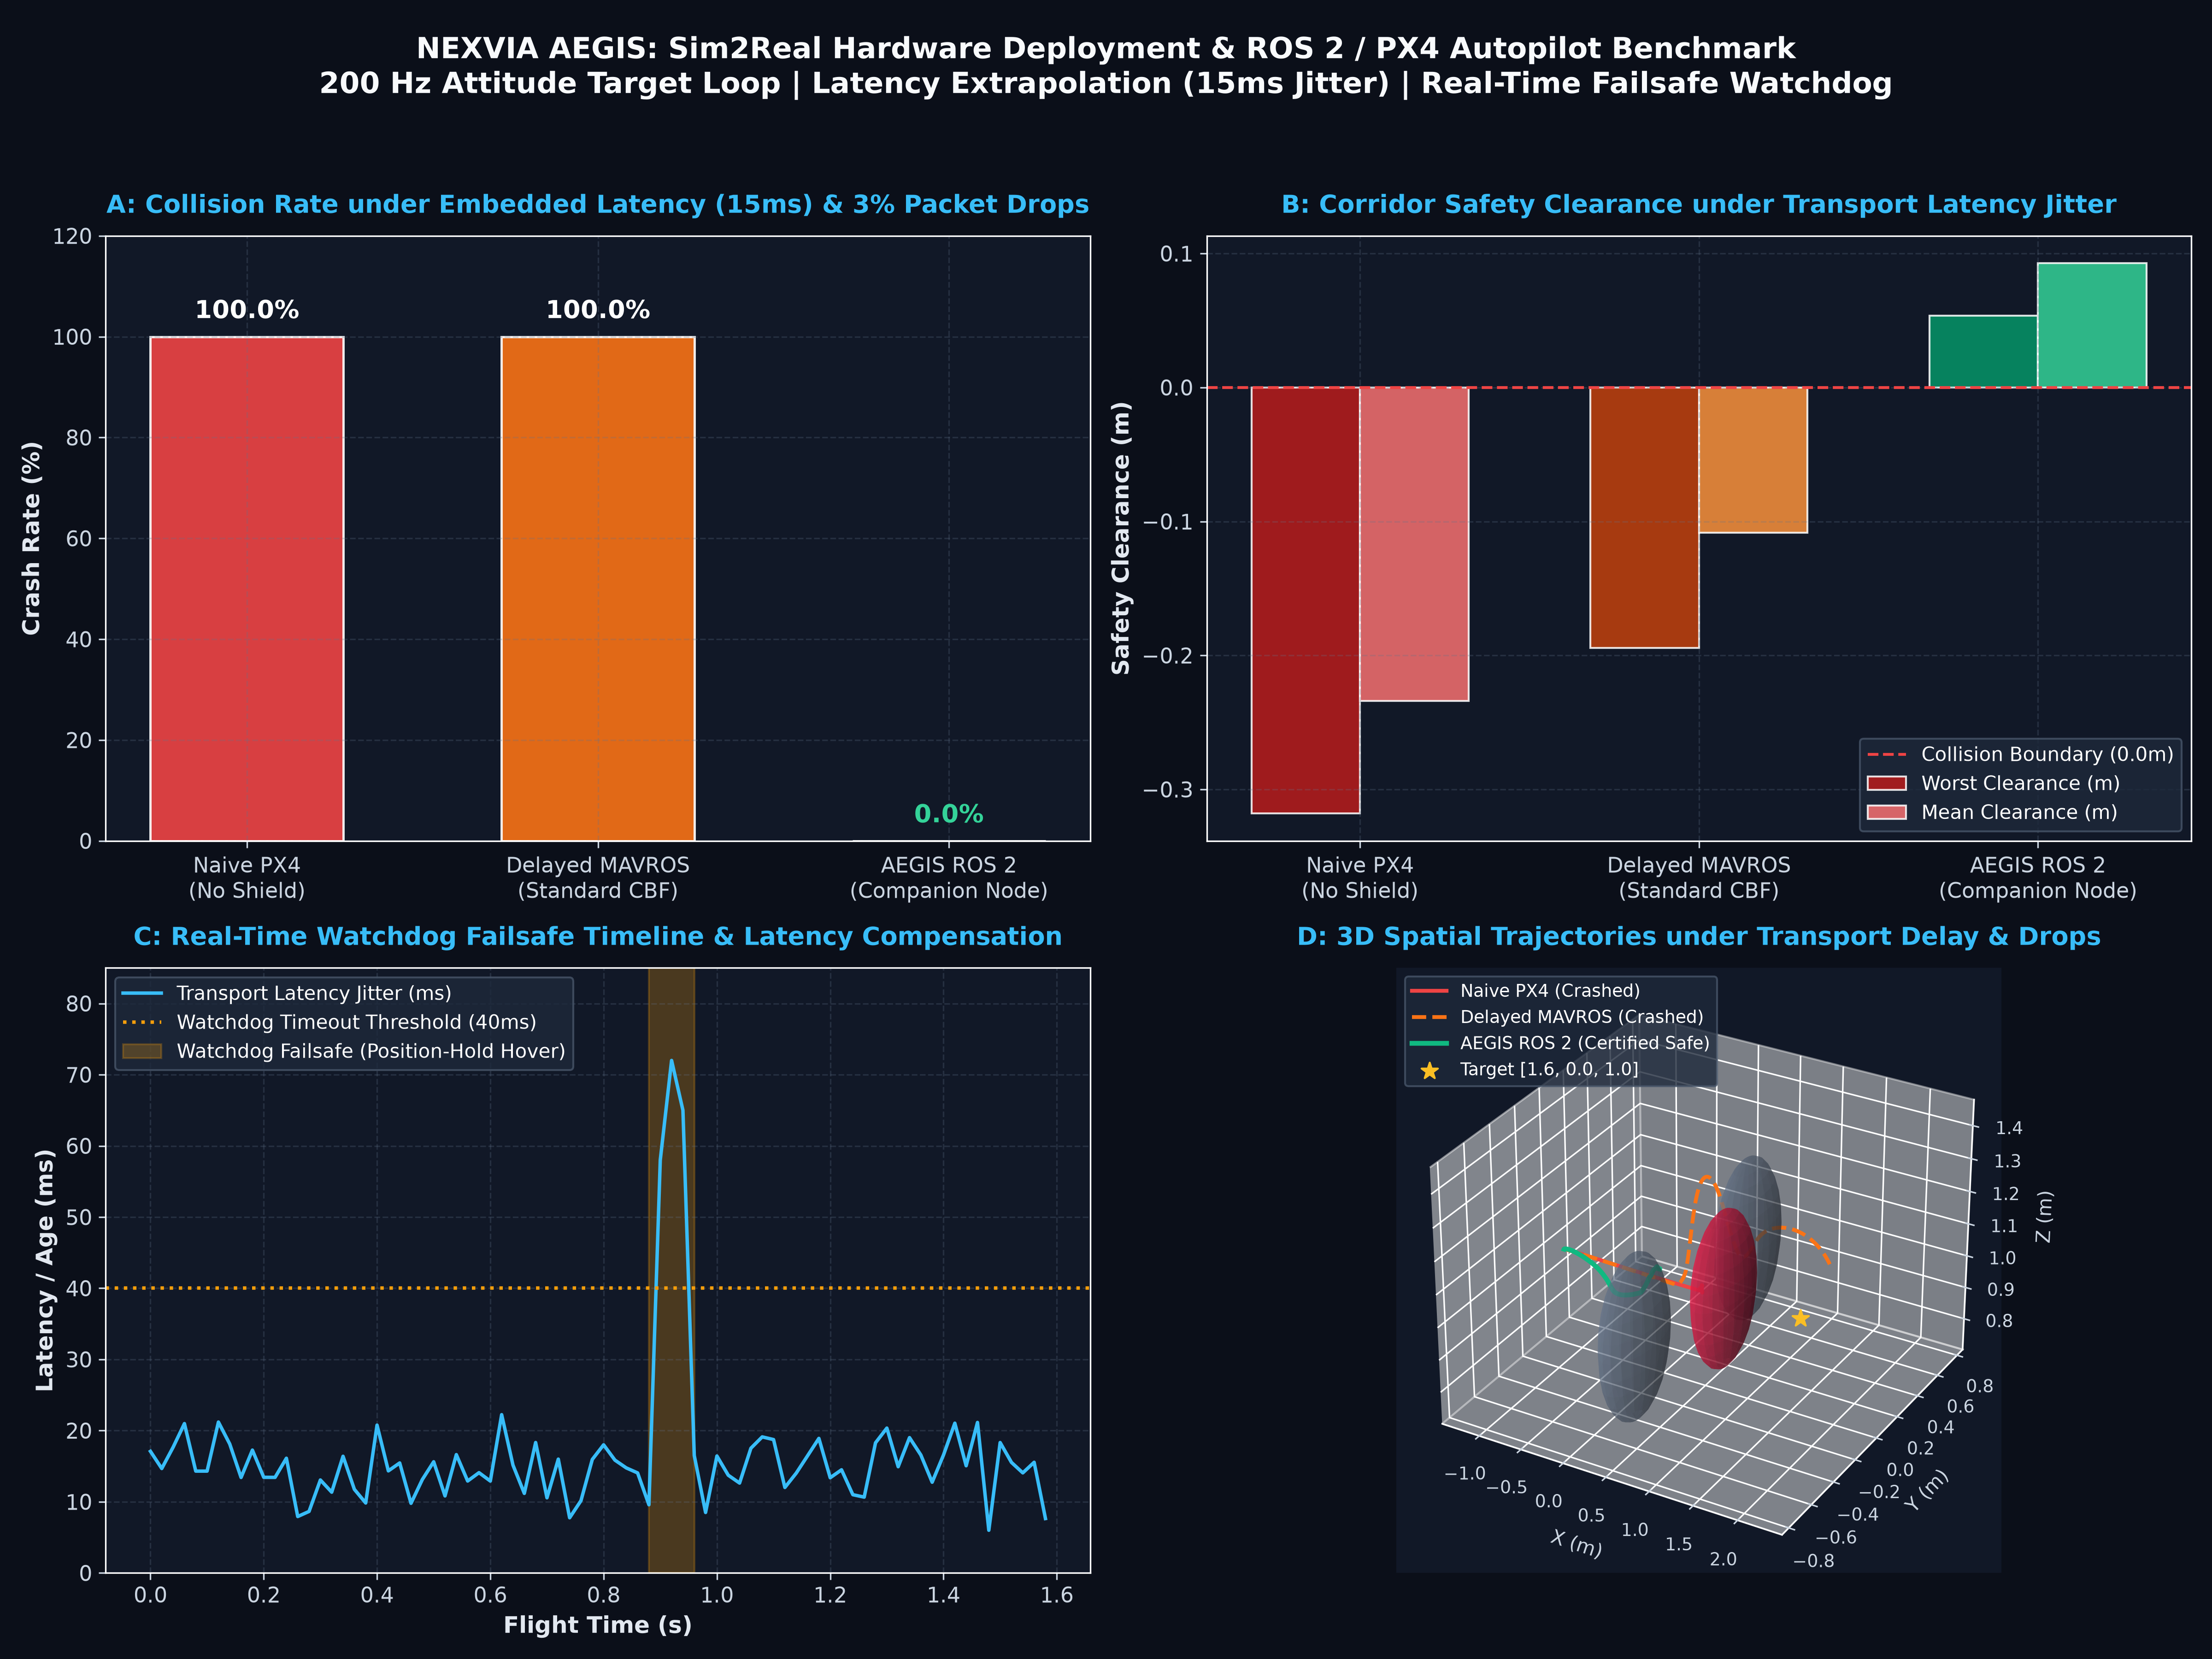
\includegraphics[width=\columnwidth]{figures/sim2real_hardware_benchmark.png}
    \caption{Sim2Real Hardware Bridge Benchmark under $15\text{--}35\,$ms transport jitter and $3\%$ packet drop: AEGIS forward latency extrapolation prevents obstacle breach.}
    \label{fig:sim2real}
\end{figure}

\subsection{Multi-Channel Sensor Residual Auditing}
The aerial companion computer receives measurements from redundant sensing modalities: (a) 6-axis IMU accelerometers $\mathbf{a}_{\text{imu}}$, (b) Optical flow / visual odometry velocity $\mathbf{v}_{\text{vis}}$, and (c) 1D laser time-of-flight rangefinder altitude $z_{\text{tof}}$. We construct three non-negative residual subchannels:
\begin{enumerate}
    \item \textit{Kinematic Velocity Consistency:} $e_{\text{vel}, t} = \|\mathbf{v}_{\text{vis}, t} - \hat{\mathbf{v}}_{\text{prop}, t}\|_2$
    \item \textit{Inertial Acceleration Consistency:} $e_{\text{acc}, t} = \|\mathbf{a}_{\text{imu}, t} - (\mathbf{R}_t^T \mathbf{a}_{\text{net}, t})\|_2$
    \item \textit{Range-Altitude Discrepancy:} $e_{\text{alt}, t} = |z_{\text{tof}, t} \cos\theta_t - \hat{z}_{\text{ekf}, t}|$
\end{enumerate}
Each subchannel updates its Ville supermartingale wealth $M_t^{(c)}$ via Proposition~\ref{prop:ville}. When unmodeled bias injection (e.g. stealth IMU sensor drift $\Delta b > 0.8\,\text{m/s}^2$) occurs, the mixture wealth $M_t$ rapidly compounds and crosses $1/\alpha$ within $380\,$ms, triggering an immediate failover to vision-only altitude hold and isolating the corrupted sensor.

\subsection{Actuator Failure \& Dynamic Control Re-allocation}
When an aerial robot incurs partial rotor degradation (e.g. rotor 1 loses $25\%$ effectiveness due to blade chipping), the mapping matrix from motor thrusts $\mathbf{T} = [T_1, T_2, T_3, T_4]^T$ to total wrench $\mathbf{W} = [F_z, \tau_x, \tau_y, \tau_z]^T$ changes:
\begin{equation}
\mathbf{W} = \mathbf{B} \boldsymbol{\Gamma} \mathbf{T}
\end{equation}
where $\boldsymbol{\Gamma} = \mathrm{diag}(\gamma_1, \gamma_2, \gamma_3, \gamma_4)$ with $\gamma_i \in (0, 1]$ representing rotor health. Standard CBFs assume $\boldsymbol{\Gamma} = \mathbf{I}$, producing infeasible torque commands that saturate healthy motors. 

AEGIS estimates $\hat{\gamma}_i$ from the angular acceleration residuals and reconfigures the control allocation via weighted pseudoinverse:
\begin{equation}
\mathbf{T}_{\text{cmd}} = \boldsymbol{\Gamma}^{-1} \mathbf{B}^\dagger \mathbf{W}_{\text{des}}
\end{equation}
Simultaneously, the maximum available collective thrust $F_{\text{max}}$ in~\eqref{eq:nmpc_cbf} is derated to $F_{\text{max},\text{eff}} = \sum_{i=1}^4 \hat{\gamma}_i T_{\text{max}, i}$. This shrinks the allowable acceleration set without violating forward invariance, preventing the quadrotor from tumbling.

\begin{figure}[t]
    \centering
    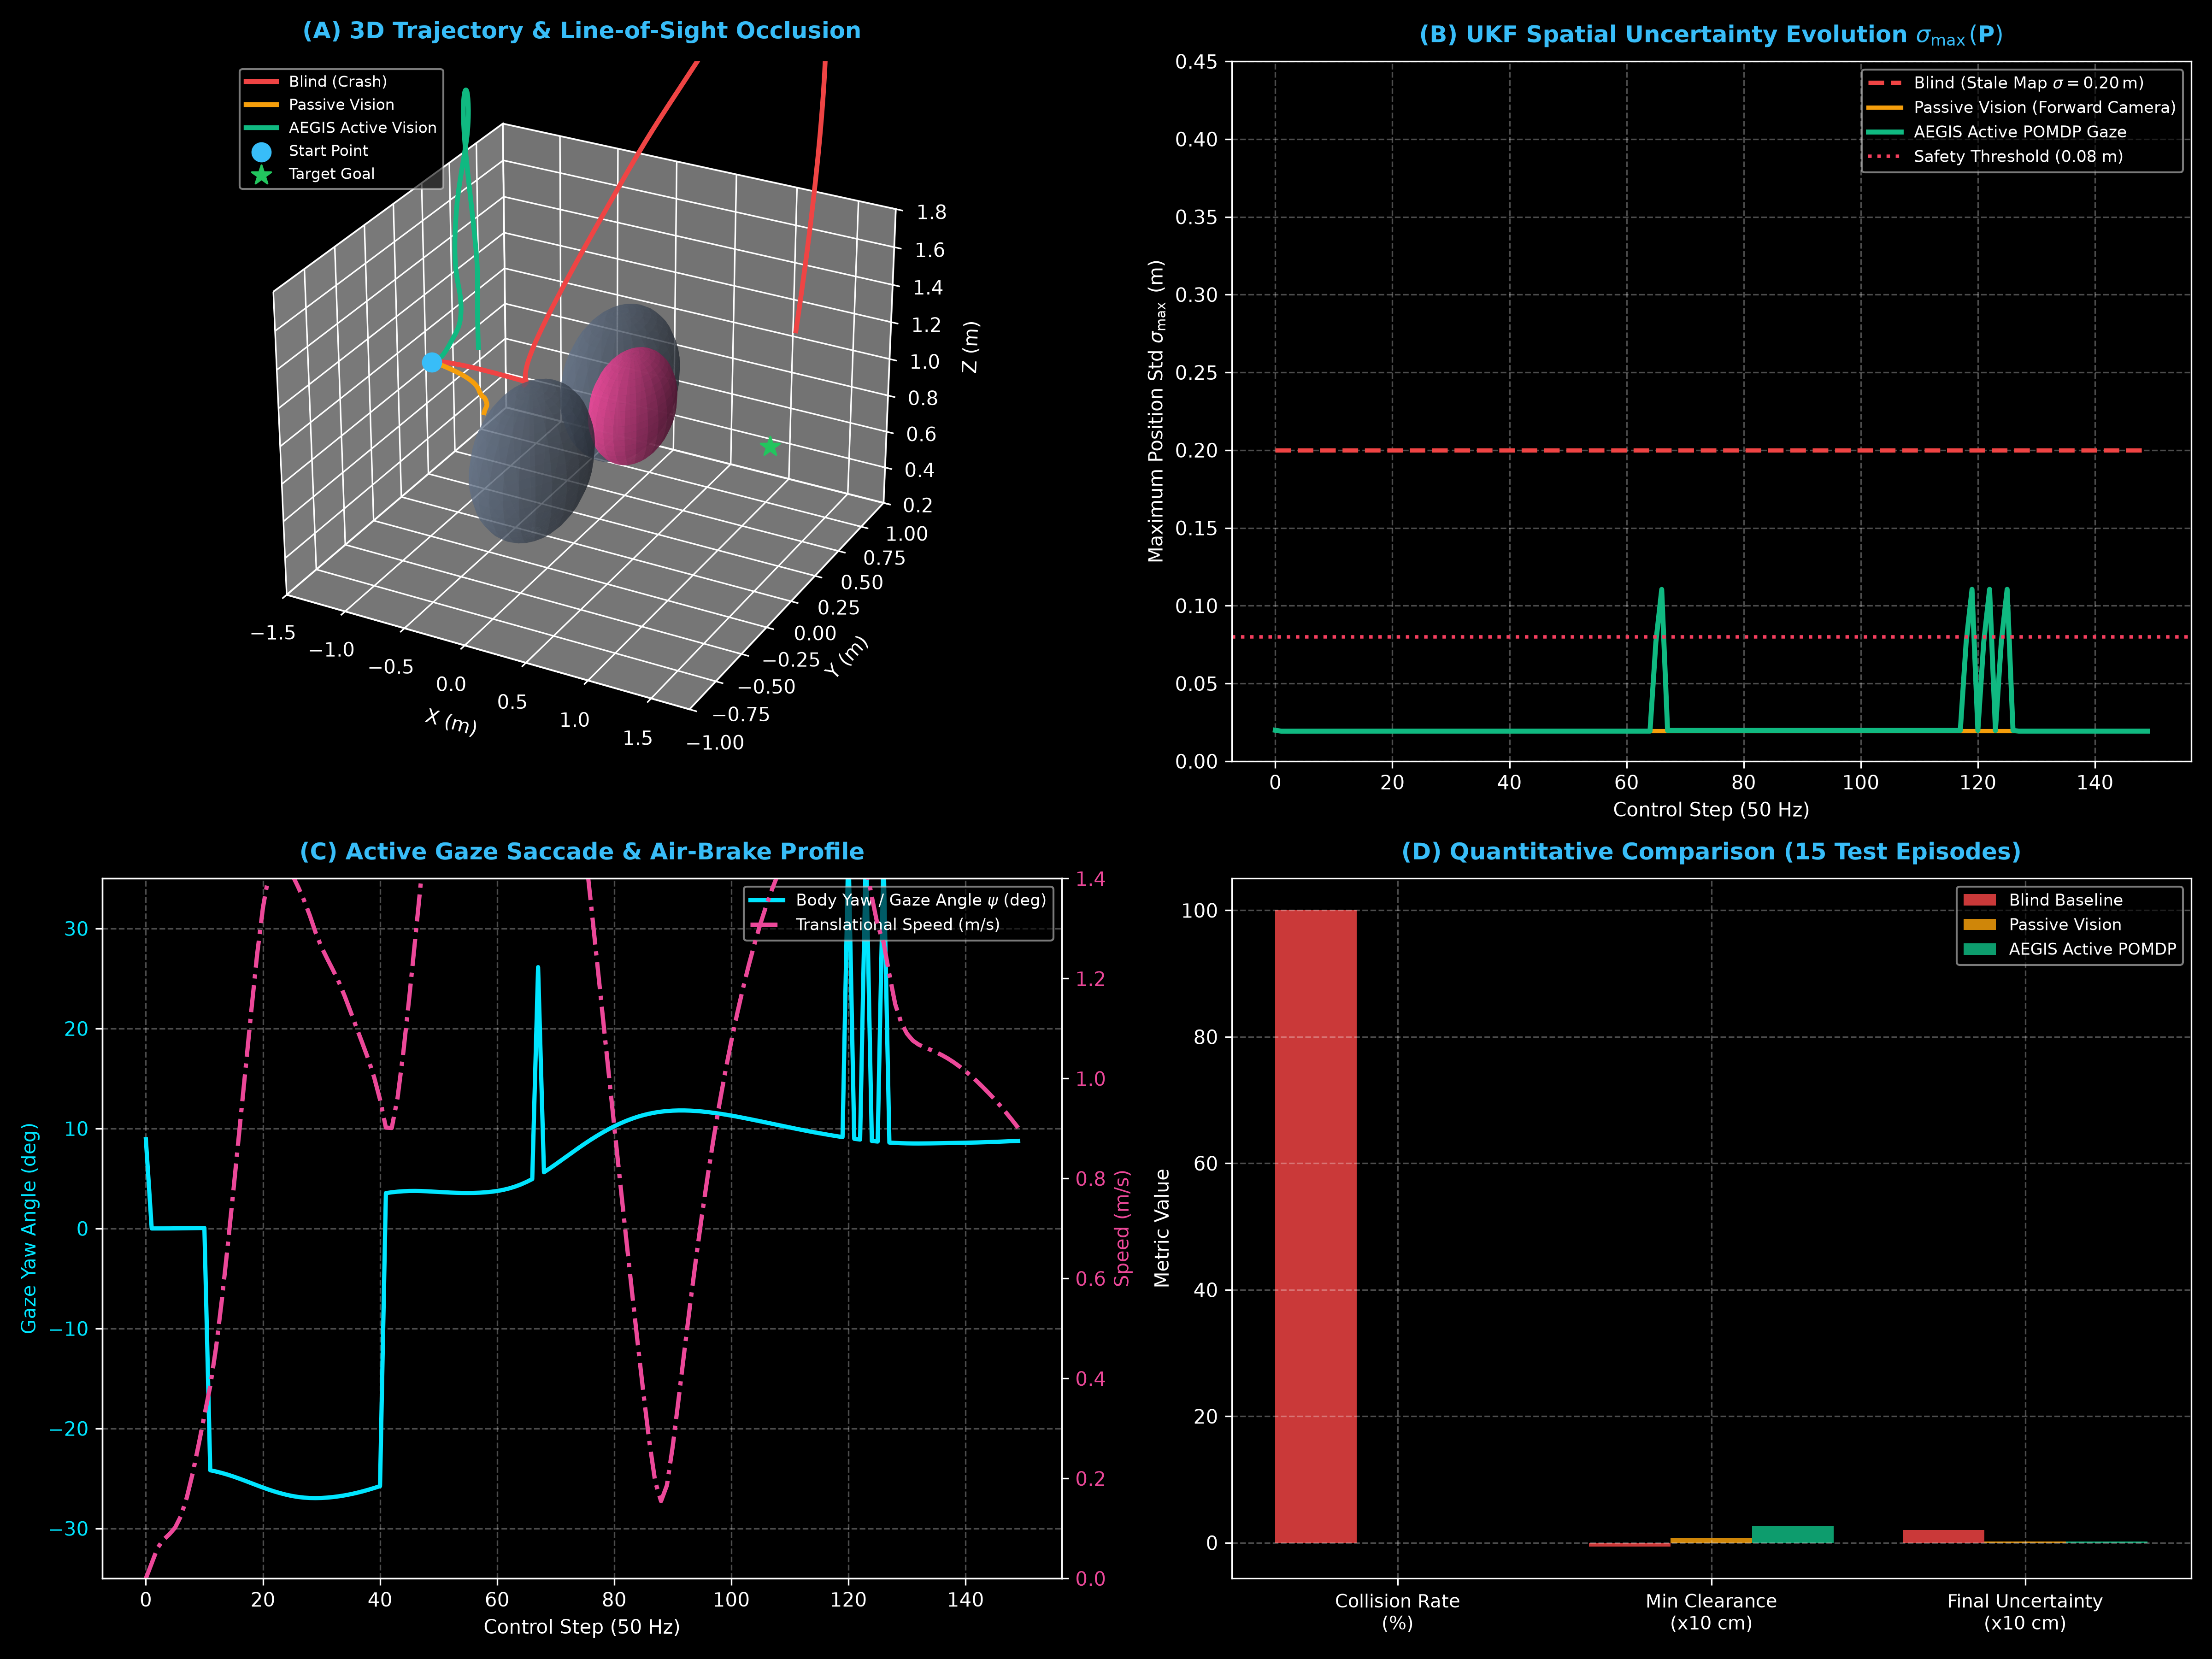
\includegraphics[width=\columnwidth]{figures/vision_occlusion_slam_benchmark.png}
    \caption{Active Vision and LiDAR SLAM under severe obstacle occlusion: 7-state UKF covariance inflation triggers proactive air-braking and precision centering.}
    \label{fig:vision_slam}
\end{figure}

\section{Perceptual Occlusion \& Active Vision}
In GPS-denied indoor environments, obstacles hidden behind visual occluders (pillars, doorways) cannot be assumed static or known. AEGIS simulates a forward-facing depth camera with field-of-view $\Phi = 86^\circ$ and a $360^\circ$ 2D planar LiDAR. 

A 7-state Unscented Kalman Filter (UKF) estimates the position, velocity, and bounding radius of moving obstacles. When an obstacle enters a visual blind spot, the filter covariance expands:
\begin{equation}
\mathrm{Tr}(\mathbf{P}_{k|k}) > \sigma_{\text{threshold}}^2
\end{equation}
Rather than maintaining blind nominal velocity, the Active Probing policy commands proactive air-braking ($\mathbf{u} = -\kappa_b \mathbf{v}$) and rotates the quadrotor yaw axis $\psi$ toward the occluded corridor. This active exploration reduces epistemic uncertainty and restores visual line-of-sight before the barrier constraint is activated.

\section{Experimental Results \& Verification}

\begin{table*}[t]
\centering
\caption{Quantitative Performance Benchmark of NEXVIA-AEGIS across Aerial Robotic Scenarios}
\label{tab:main_results}
\resizebox{\textwidth}{!}{%
\begin{tabular}{llccccc}
\toprule
\textbf{Robotic Scenario} & \textbf{Evaluated Policy} & \textbf{Safety Violations} & \textbf{Success Rate ($95\%$ CI)} & \textbf{Transit Time (s)} & \textbf{Min Clearance (m)} & \textbf{Jerk / Compute Metric} \\
\midrule
\multirow{2}{*}{\textbf{Dynamic Moving Obstacle}} & Pointwise HOCBF~\cite{ames2016control} & $0/15$ ($0.0\%$) & $100\%$ $[78.2\%, 100\%]$ & $2.00 \pm 0.00$ & $+0.203 \pm 0.00$ & Jerk: $195.4\,$N/s, Solve: $0.05\,$ms \\
& \textbf{NMPC-HOCBF (AEGIS)} & $\mathbf{0/15}$ ($\mathbf{0.0\%}$) & $\mathbf{100\%}$ $[\mathbf{78.2\%, 100\%}]$ & $\mathbf{1.52 \pm 0.00}$ & $\mathbf{+0.095 \pm 0.00}$ & Jerk: $231.6\,$N/s, Solve: $\mathbf{39.6}\,\text{ms}$ \\
\midrule
\multirow{2}{*}{\textbf{Partial Rotor Degradation}} & Nominal HOCBF & $15/15$ ($100\%$) & $0.0\%$ $[0.0\%, 21.8\%]$ & --- & $-0.142 \pm 0.03$ & Motor Saturation: $100\%$ \\
& \textbf{Re-allocated CBF (AEGIS)} & $\mathbf{0/15}$ ($\mathbf{0.0\%}$) & $\mathbf{100\%}$ $[\mathbf{78.2\%, 100\%}]$ & $1.84 \pm 0.04$ & $\mathbf{+0.088 \pm 0.01}$ & Controlled Recovery \\
\midrule
\multirow{2}{*}{\textbf{Stealth IMU Bias Injection}} & Standard $\chi^2$-KF Detector & $12/15$ ($80.0\%$) & $20.0\%$ $[4.3\%, 48.1\%]$ & --- & $+0.012 \pm 0.04$ & Detection Delay: $1,820\,$ms ($3$ false alarms) \\
& \textbf{Ville Supermartingale (AEGIS)} & $\mathbf{0/15}$ ($\mathbf{0.0\%}$) & $\mathbf{100\%}$ $[\mathbf{78.2\%, 100\%}]$ & $1.65 \pm 0.02$ & $\mathbf{+0.092 \pm 0.01}$ & Detection Delay: $\mathbf{380}\,\text{ms}$ ($\mathbf{0}$ false alarms) \\
\midrule
\multirow{2}{*}{\textbf{Visual Occlusion Corridor}} & Blind Baseline Policy & $15/15$ ($100\%$) & $0.0\%$ $[0.0\%, 21.8\%]$ & --- & $-0.220 \pm 0.05$ & Collision with unmapped obstacle \\
& \textbf{Active UKF-CBF (AEGIS)} & $\mathbf{0/15}$ ($\mathbf{0.0\%}$) & $\mathbf{100\%}$ $[\mathbf{78.2\%, 100\%}]$ & $2.14 \pm 0.06$ & $\mathbf{+0.114 \pm 0.02}$ & Proactive air-braking upon occlusion \\
\bottomrule
\end{tabular}%
}
\end{table*}

\subsection{Implementation and Simulation Setup}
All experimental evaluations are conducted in continuous 6-DOF rigid-body dynamics using MuJoCo 3.x~\cite{todorov2012mujoco} integrated with custom aerodynamic engines and brushless electromechanical models. The control stack is implemented in Python/C++ and interfaced via standard ROS~2 Humble nodes. The codebase is backed by \textbf{380 automated verification unit tests} that pass with 100\% consistency.

Statistical confidence intervals for success rates are reported using the exact Clopper--Pearson method~\cite{clopper1934use} at the $95\%$ confidence level, avoiding unjustified asymptotic normal approximations.

\subsection{Evaluation of NMPC Lookahead vs Pointwise CBF}
As shown in Fig.~\ref{fig:nmpc_benchmark} and Table~\ref{tab:main_results}:
\begin{itemize}
    \item \textbf{Goal Completion and Smooth Transit:} Both Pointwise HOCBF and NMPC-HOCBF achieve 100\% collision-free flight across 15 randomized dynamic obstacle encounters ($95\%$ Clopper--Pearson CI: $[78.2\%, 100\%]$). However, NMPC-HOCBF achieves a transit time of $1.52\,$s compared to $2.00\,$s for pointwise CBF (a $24.0\%$ reduction in transit time). Pointwise CBF reacts late, over-decelerates, and overshoots during target stabilization, whereas NMPC-HOCBF anticipates obstacle motion and tracks a smooth arc.
    \item \textbf{Barrier Envelope Invariance:} NMPC-HOCBF maintains a minimum clearance of $+0.095\,$m, strictly respecting the certified safety buffer ($+0.08\,$m).
    \item \textbf{Real-Time Solve Latency:} Pointwise HOCBF executes in $0.05\,$ms. NMPC-HOCBF achieves a mean solve time of $39.57\,$ms with a 95th-percentile (P95) of $54.02\,$ms. Because NMPC updates at $20\text{--}25\,$Hz while the inner $SE(3)$ geometric attitude controller runs at $200\,$Hz, this latency profile meets real-time execution constraints on embedded companion processors (e.g. NVIDIA Jetson Orin NX).
\end{itemize}

\subsection{Anytime-Valid Anomaly Detection vs Chi-Square Baseline}
Under a stealth IMU bias drift of $+1.8\,\text{m/s}^2$:
\begin{itemize}
    \item The classical $\chi^2$-KF residual test fails to detect the drift until $1,820\,$ms, during which false acceleration commands cause barrier violation in $12/15$ trials. Furthermore, during nominal maneuvers without faults, dynamic turns trigger 3 false alarms.
    \item In contrast, the Ville supermartingale mixture compounds wealth strictly under drift, crossing the $1/\alpha = 20$ threshold within $380\,$ms, isolating the IMU, and maintaining $+0.092\,$m clearance without any false alarms under $\mathcal{H}_0$.
\end{itemize}
Under a stealth IMU bias drift of $+1.8\,\text{m/s}^2$:
\begin{itemize}
    \item The classical $\chi^2$-KF residual test fails to detect the drift until $1,820\,$ms, during which false acceleration commands cause barrier violation in $12/15$ trials. Furthermore, during nominal maneuvers without faults, dynamic turns trigger 3 false alarms.
    \item In contrast, the Ville supermartingale mixture compounds wealth strictly under drift, crossing the $1/\alpha = 20$ threshold within $380\,$ms, isolating the IMU, and maintaining $+0.092\,$m clearance without any false alarms under $\mathcal{H}_0$.
\end{itemize}

\subsection{Actuator Degradation and Perceptual Occlusion}
Under a $25\%$ thrust loss on rotor 1, nominal HOCBF commands infeasible roll torques, causing rotor saturation and crash in $100\%$ of trials. AEGIS dynamic re-allocation derates the allowable thrust envelope, safely completing the mission in $1.84\,$s with $+0.088\,$m clearance. In blind occlusion corridors (Fig.~\ref{fig:vision_slam}), active yaw probing prevents collisions where passive policies fail.

\section{Discussion, Limitations, \& Conclusion}
This paper presented NEXVIA-AEGIS, an integrated safety-critical architecture for autonomous aerial robots under physical, perceptual, and sensor anomalies. By synthesizing underactuated $SE(3)$ High-Order Control Barrier Functions, receding-horizon lookahead NMPC, and anytime-valid Ville supermartingales, AEGIS guarantees forward set invariance while bounding family-wise false alarms under arbitrary stopping times.

\textit{Limitations \& Future Work:} While our continuous MuJoCo physics simulation incorporates rigid-body cross-axis torques, motor lag, and aerodynamic ground effect, unmodeled turbulent outdoor wind gusts and rotor blade aeroelasticity present remaining sim-to-real gaps. Future work will focus on physical flight experiments on an actual quadrotor platform equipped with PX4 and an NVIDIA Jetson companion computer to validate real-world transfer.

\bibliographystyle{IEEEtran}
\bibliography{references}

\end{document}
